\documentclass{article}
\usepackage[utf8]{inputenc}
\usepackage{graphicx}
\usepackage{hyperref}
\usepackage[nonumberlist,nopostdot]{glossaries}

\title{Modern MVC web framework in Golang}
\author{Senior design project (Spring 2016--Fall 2016)}
\date{\today}
\makeglossaries

\begin{document}

\maketitle

\section{Introduction}

The project is to design and build a framework based on the Model-View-Controller (\textsc{mvc}) design paradigm to improve the process of developing web applications in Golang. Golang, also referred to as Go, is an open source programming language developed at Google that emphasizes concurrency and safety. Since the language’s inception in 2009, Go has been quickly gaining popularity for use on high-performance, concurrent servers. The web framework to be designed would address the need of web developers to quickly bootstrap and reliably maintain web applications in Go. At its core, the framework would provide developers a command-line \textsc{api} to generate the controllers, views, and models required to build their complex web applications.  The project involves the challenges of architecting a large software application; routing \textsc{http} requests concurrently and securely; linking models, views, and controllers; and providing a unified interface for database queries. The components of the application would be tested continuously throughout the development cycle using unit tests and continuous integration (\textsc{ci}). Documentation to use the framework and an example web application built using the framework will also be included. 

\section{MVC and the web}

The Model-View-Controller (\textsc{mvc}) design paradigm suits the development of web applications. Most user-facing web applications need to perform the following tasks: store, persist, and retrieve user data (Model); handle and route user requests to manipulate the data (Controller); and represent information to the user in a variety of formats---\textsc{html, json}, etc. (View). 

\subsection{Scalability and the need for frameworks in more languages}

Most of the popular frameworks that have emerged in the past decade are made for dynamically typed languages. They include Ruby on Rails (for the Ruby programming language), Django (for Python), and Sails.js (for JavaScript). However, large projects written in scripting languages such as Ruby, Python, and JavaScript without type-checking are unwieldy to maintain and difficult to scale, as many companies such as Twitter have discovered.\footnote{{https://blog.twitter.com/2011/the-engineering-behind-twitter-s-new-search-experience}}

As a result, more performant languages such as Java, Scala, and C\texttt{++} continue to be used by large companies for their backend infrastructures. Go is an upcoming language that belongs to this category.

\subsection{Golang MVC frameworks}

Go currently has a few third-party libraries that facilitate developing web applications---most are fairly lightweight and some follow the \textsc{mvc} paradigm. Gorilla and Martini are two popular libraries, but they make a conscious effort to be lightweight (in fact, Gorilla is just a collection of discrete packages). Beego and Revel are other Golang based \textsc{mvc} framework solutions. 

\section{Technical details}

The project would be an exercise in best practices in concurrency, \textsc{http} specifications, \textsc{rest} principles, web security, databases, web application development, writing forward-thinking \textsc{api}s, and developing as a community. Experience or familiarity in these areas is a plus.

\subsection{Development}

The majority of the project will be developed using the latest stable release of Go, which currently is \texttt{go1.6}. 

\begin{figure}[h]
\centering
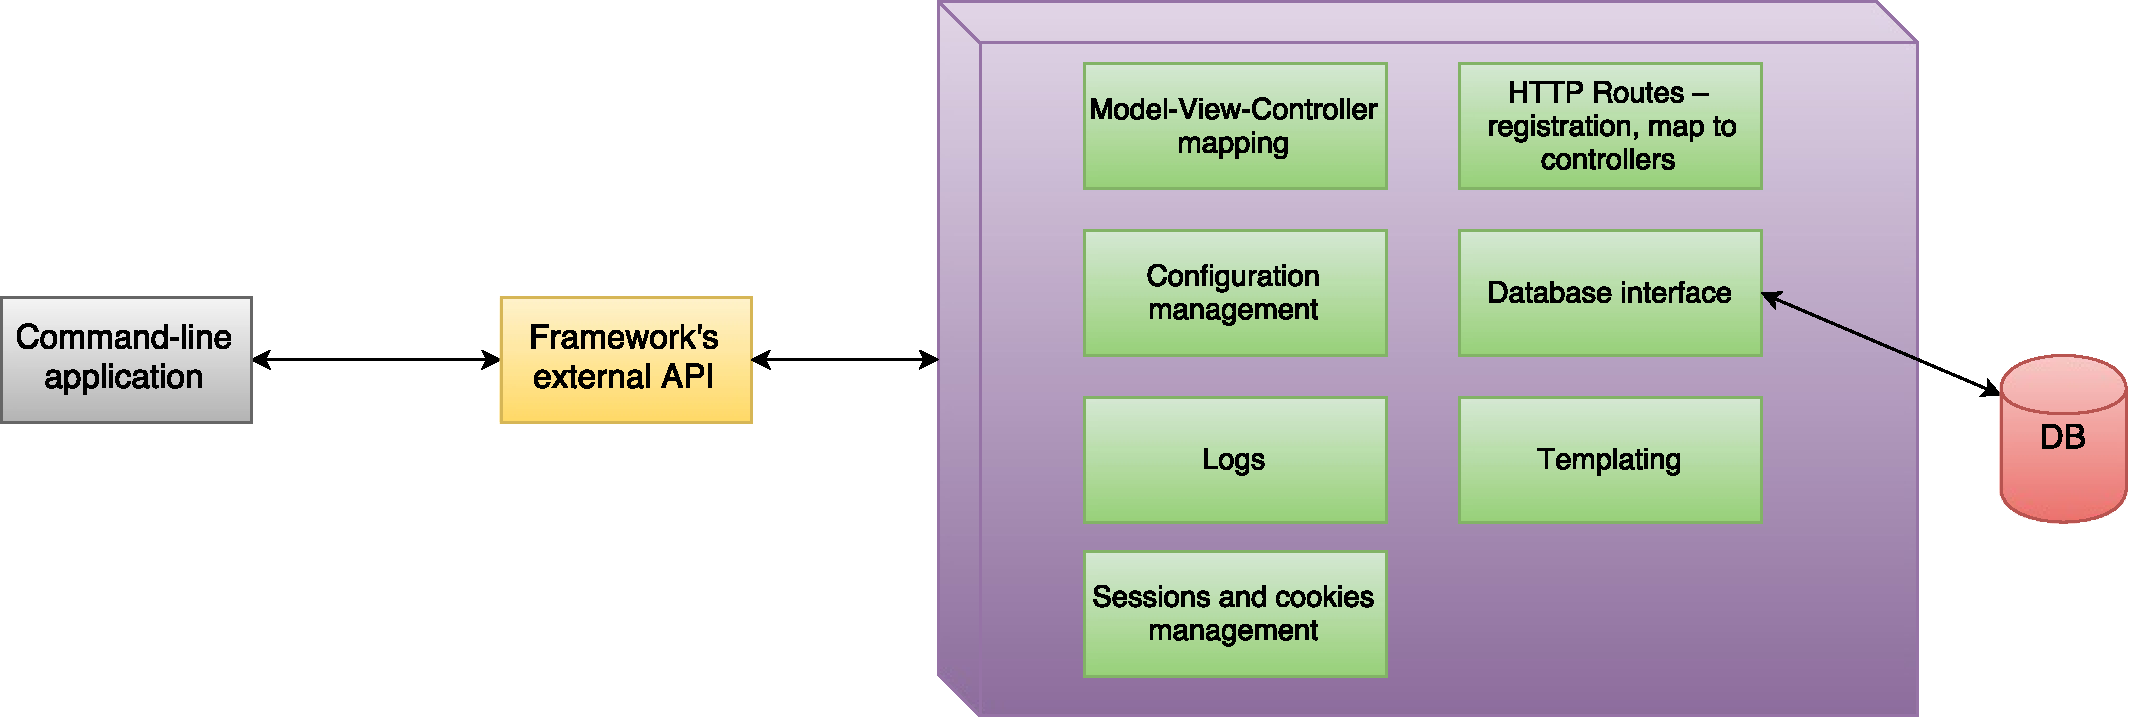
\includegraphics[width=1.1\textwidth]{mvc-app.pdf}
\caption{Major framework components }
\end{figure}

The major components are:

\begin{itemize}
    \item \textbf{The base of the framework}: This includes code for generating files for the requested models, views, and controllers. It also involves rules for mapping related models, views, and controllers and maintaining these relationships through the lifetime of the application.
    \item \textbf{Command-line application}: The command-line interface will provide the developer access to the framework's \textsc{api}. It would allow developers to start and stop the server; generate new models, views, and controllers; configure their application; and deploy their application.
    \item \textbf{Server, router, sessions}: The framework would come with a built-in \textsc{http} server to serve applications. The plan is to make components easily swappable, so developers can choose to drop in their own \textsc{http} server, mux, or router implementation during production if needed. This would rely on Go's \texttt{net/http} package or on faster alternatives such as \texttt{valyala/fasthttp}.\footnote{The open source package available at {https://github.com/valyala/fasthttp} claims to be up to 10x faster than the built-in http package} The other related components include the router and a cookies and sessions manager. 
    \item \textbf{Database interface}: Models would need to persist on disk. Developing a domain specific query language (\textsc{dsl}) would abstract away the details of the underlying database from application developers. The interface would provide a unified way of accessing the database and make it possible to replace the underlying database safely without significant developer effort.
    \item \textbf{Templating engine}: This is required to render model data on \textsc{html} views. As of now, Go's \texttt{html/template} package appears to be a good choice---providing a good balance of performance, familiarity to users, and support for expressive programming logic directly in the view templates.
\end{itemize}

\begin{figure}[h]
\centering
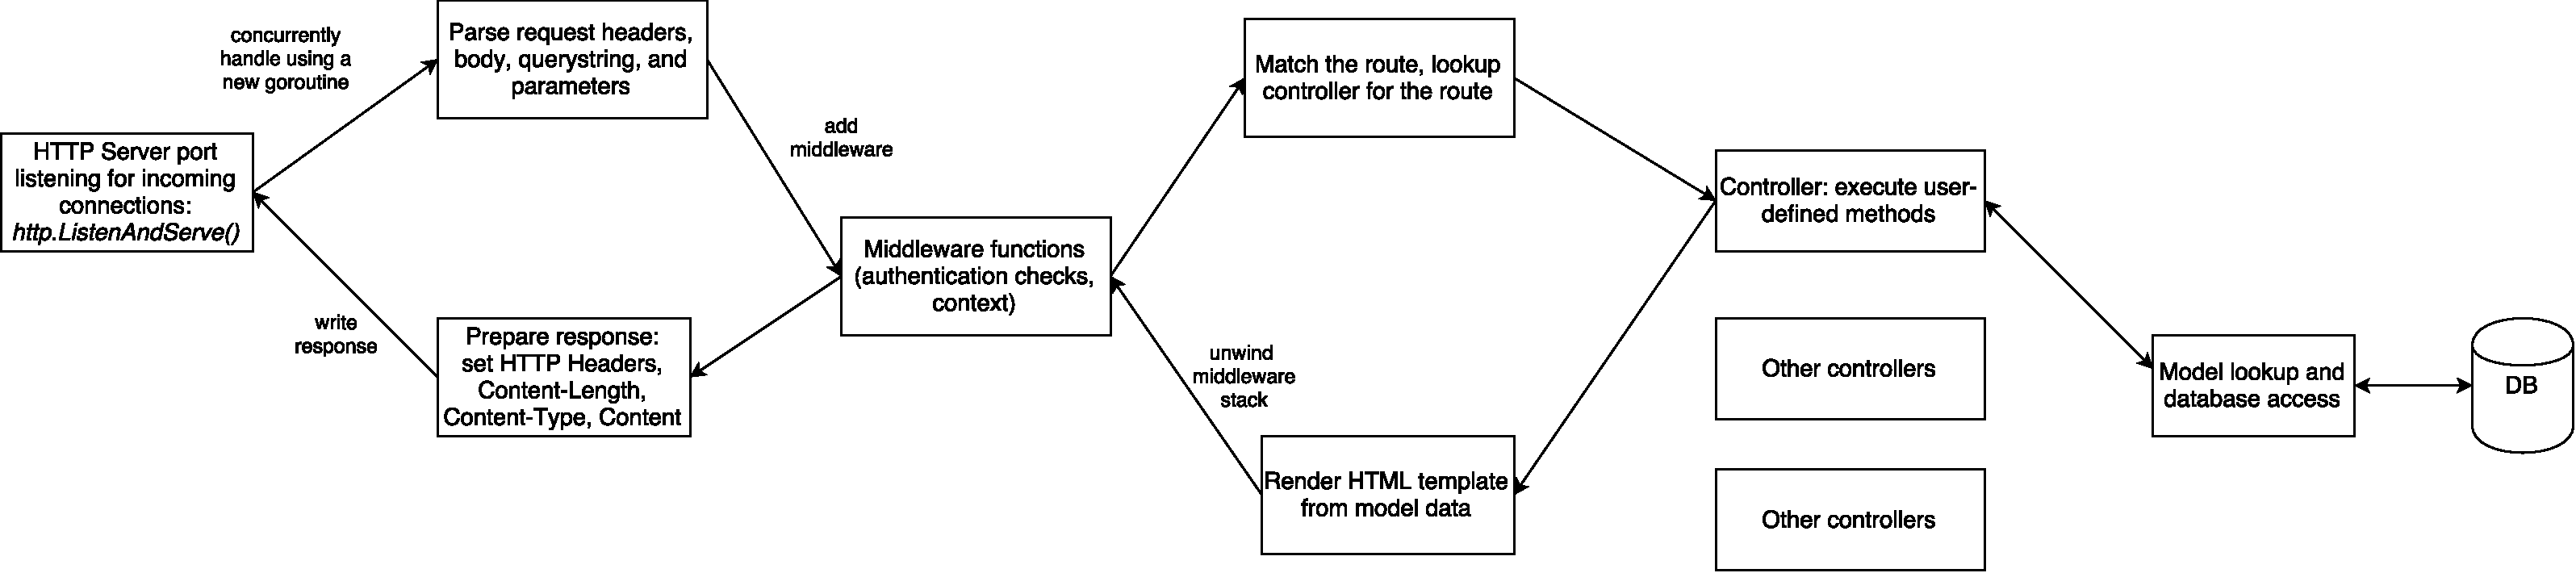
\includegraphics[width=1.1\textwidth]{mvc-run.pdf}
\caption{Framework runtime: handling a simple request}
\end{figure}

\subsection{Extras}

The project will include support for easy integration of:

\begin{itemize}
    \item Authentication with common log-in providers such as Google, Gravatar, Twitter, and GitHub.
    \item Third-party data persistence solutions such as Firebase, Google Cloud DataStore, and AppEngine DataStore.
    \item Deployment to Heroku, Digital Ocean, and Amazon Web Services.
    \item Support for in memory data storage systems such as Redis.
    \item Testing and load generation tools.
\end{itemize}

\subsection{Lines of code}

The team anticipates that the project will require around 20,000 lines of code.

\subsection{Testing}

Code coverage is an important component of the project. Unit tests will be written when appropriate. The plan is to use continuous integration and build system solutions such as TravisCI and Wercker to trigger tests and builds on each commit.

\section{Challenges}

From initial discussions, the team currently expects these challenges:

\begin{itemize}
    \item \textbf{Architecting the framework}: The framework comprises of several distinct components which would need to be developed in parallel and integrated. The framework would need to be architected in a manner that is maintainable and flexible enough to modify on the long term.
    \item \textbf{Connecting related models, views, controllers}: Naming conventions (à la Rails style) or developer configurable options should exist for mapping relations between routes, controllers, models, and views. The pros and cons of either approach need to be evaluated. Finally, the implementation would need to be error- and ambiguity-free, as this is a part of the framework's logic that will be used on every incoming request for standard applications.
\end{itemize}

Thoughtful design decisions in the initial stages are important for the success of the project. Research on the beneficial parts of and criticism on existing \textsc{mvc} frameworks (including those written in other languages), and careful problem scoping should address most issues. The team would also need to spend time to get acquainted with the Go programming language.

\section{Costs}

The team does not anticipate major financial costs in the development of the framework. 

\section{Conclusion}

The team is currently in the design phase---researching existing designs, evaluating prospective tools, and formulating the architecture for the framework. Feedback and suggestions are always welcome.\\


Contact for questions, comments regarding this proposal: 

\begin{itemize}
    \item Joshua Dong $\langle jdong42@gmail.com \rangle$
    \item Brad Gray $\langle bpgray@utexas.edu \rangle$
    \item *Rahul Jaisimha $\langle rahul@jaisimha.com \rangle$
    \item Salim Memon $\langle salim.memon@utexas.edu  \rangle$
    \item *Taiyi Ouyang $\langle taiyi.o@utexas.edu \rangle$
    \item *Nishanth Shanmugham $\langle nishanths@utexas.edu \rangle$
\end{itemize}

Students marked with * are honors students.

% Glossary
\newglossaryentry{api}
{
  name=API,
  description={
    Application Programming Interface. Defines an interface that software programs can use to interact
  }
}

\newglossaryentry{mvc}
{
  name=MVC,
  description={
    Model View Controller. A design paradigm in software engineering. Suitable for the design of web applications.
  }
}

\newglossaryentry{ci}
{
  name=CI,
  description={
    Continuous Integration. A software development strategy in which code that is committed is tested and integrated using automation tools to catch errors early.
  }
}

\newglossaryentry{http}
{
  name=HTTP,
  description={
    Hypertext Transfer Protocol. The network protocol that is the basis of communication on the World Wide Web.
  }
}

\newglossaryentry{rest}
{
  name=REST,
  description={
    Representational State Transfer. An architectural style for web application design and resource handling. RESTful systems emphasize statelessness and generally communicate over HTTP.
  }
}

\newglossaryentry{rails}
{
  name=Rails,
  description={
    Ruby on Rails, or Rails for short, is an MVC web development framework for the Ruby programming language.
  }
}

\newglossaryentry{digitalocean}
{
  name=Digital Ocean,
  description={
    A cloud services infrastructure provider.
  }
}

\newglossaryentry{firebase}
{
  name=Firebase,
  description={
    An online, easy-to-configure database service company.
  }
}

\newglossaryentry{redis}
{
  name=Redis,
  description={
    A high-performance, in-memory data structure store commonly used for caching. 
  }
}

\newglossaryentry{appengine}
{
  name=AppEngine,
  description={
    A web application hosting platform from Google
  }
} 

\newglossaryentry{heroku}
{
  name=Heroku,
  description={
    A web application hosting company.
  }
}



\glsaddall
\printglossaries

\end{document}